% Options for packages loaded elsewhere
\PassOptionsToPackage{unicode}{hyperref}
\PassOptionsToPackage{hyphens}{url}
\documentclass[
]{article}
\usepackage{xcolor}
\usepackage[margin=1in]{geometry}
\usepackage{amsmath,amssymb}
\setcounter{secnumdepth}{-\maxdimen} % remove section numbering
\usepackage{iftex}
\ifPDFTeX
  \usepackage[T1]{fontenc}
  \usepackage[utf8]{inputenc}
  \usepackage{textcomp} % provide euro and other symbols
\else % if luatex or xetex
  \usepackage{unicode-math} % this also loads fontspec
  \defaultfontfeatures{Scale=MatchLowercase}
  \defaultfontfeatures[\rmfamily]{Ligatures=TeX,Scale=1}
\fi
\usepackage{lmodern}
\ifPDFTeX\else
  % xetex/luatex font selection
\fi
% Use upquote if available, for straight quotes in verbatim environments
\IfFileExists{upquote.sty}{\usepackage{upquote}}{}
\IfFileExists{microtype.sty}{% use microtype if available
  \usepackage[]{microtype}
  \UseMicrotypeSet[protrusion]{basicmath} % disable protrusion for tt fonts
}{}
\makeatletter
\@ifundefined{KOMAClassName}{% if non-KOMA class
  \IfFileExists{parskip.sty}{%
    \usepackage{parskip}
  }{% else
    \setlength{\parindent}{0pt}
    \setlength{\parskip}{6pt plus 2pt minus 1pt}}
}{% if KOMA class
  \KOMAoptions{parskip=half}}
\makeatother
\usepackage{longtable,booktabs,array}
\newcounter{none} % for unnumbered tables
\usepackage{calc} % for calculating minipage widths
% Correct order of tables after \paragraph or \subparagraph
\usepackage{etoolbox}
\makeatletter
\patchcmd\longtable{\par}{\if@noskipsec\mbox{}\fi\par}{}{}
\makeatother
% Allow footnotes in longtable head/foot
\IfFileExists{footnotehyper.sty}{\usepackage{footnotehyper}}{\usepackage{footnote}}
\makesavenoteenv{longtable}
\usepackage{graphicx}
\makeatletter
\newsavebox\pandoc@box
\newcommand*\pandocbounded[1]{% scales image to fit in text height/width
  \sbox\pandoc@box{#1}%
  \Gscale@div\@tempa{\textheight}{\dimexpr\ht\pandoc@box+\dp\pandoc@box\relax}%
  \Gscale@div\@tempb{\linewidth}{\wd\pandoc@box}%
  \ifdim\@tempb\p@<\@tempa\p@\let\@tempa\@tempb\fi% select the smaller of both
  \ifdim\@tempa\p@<\p@\scalebox{\@tempa}{\usebox\pandoc@box}%
  \else\usebox{\pandoc@box}%
  \fi%
}
% Set default figure placement to htbp
\def\fps@figure{htbp}
\makeatother
\setlength{\emergencystretch}{3em} % prevent overfull lines
\providecommand{\tightlist}{%
  \setlength{\itemsep}{0pt}\setlength{\parskip}{0pt}}
\usepackage{float}
\usepackage{booktabs}
\usepackage{longtable}
\usepackage{caption}
\captionsetup{font=small, labelfont=bf}
\let\Bbbk\relax    
\let\arrowvert\relax  
\let\arrowdblvert\relax
\usepackage{fontspec}
\setmainfont{Times New Roman} % o
\setsansfont{Arial}  
\setmonofont{Courier New}  
\usepackage{amsmath, amssymb, amsfonts}
\usepackage{graphicx}
\usepackage{booktabs}
\usepackage{longtable}
\usepackage{array}
\usepackage{multirow}
\usepackage{wrapfig}
\usepackage{float}
\usepackage{colortbl}
\usepackage{pdflscape}
\usepackage{tabu}
\usepackage{threeparttable}
\usepackage{threeparttablex}
\usepackage[normalem]{ulem}
\usepackage{makecell}
\usepackage{xcolor}
\usepackage{bookmark}
\IfFileExists{xurl.sty}{\usepackage{xurl}}{} % add URL line breaks if available
\urlstyle{same}
\hypersetup{
  pdftitle={Arsenal Season Stats{,} EPL '24-'25},
  hidelinks,
  pdfcreator={LaTeX via pandoc}}

\title{Arsenal Season Stats, EPL '24-'25}
\author{}
\date{\vspace{-2.5em}}

\begin{document}
\maketitle

{
\setcounter{tocdepth}{2}
\tableofcontents
}
\subsection{Overview}\label{overview}

A(r)senal Analysis is an analytical exploration of Arsenal's performance
in the \textbf{2024-2025} season of the \textbf{English Premier League}.
The team was chosen because of their ability to outperform league
leaders and top contenders in the UEFA Champion's League (particularly
their 3-0 win over Real Madrid) yet showing recurring inconsistencies in
front of goal.

Throughout the season, fans and pundits alike heralded it as
\emph{``Arsenal's year.''} With Manchester City's dominance waning, the
path to the title seemed open. Yet by May, Liverpool sat atop the table
while Arsenal once again finished second. The central question, then, is
this: how can a squad strong enough to reach the Champions League
semi-finals and challenge England's best still struggle to convert that
dominance into goals?

\subsection{Research Questions}\label{research-questions}

\begin{itemize}
\tightlist
\item
  What factors contribute to Arsenal's inconsistent domestic
  performance, despite victories over top-tier teams like Real Madrid
  and Manchester City?
\item
  To what extent do expected goals (xG) and expected goals against (xGA)
  reliably predict actual team outcomes?
\item
  How does Arsenal's goal-scoring distribution among players impact
  their overall offensive effectiveness?
\end{itemize}

\subsection{Methodology}\label{methodology}

I scraped aggregated match data from FBRef and used Kaggle datasets for
player-level statistics and the official fixture list. The datasets were
stored in a Docker-based MariaDB instance in my homelab for reproducible
querying. Using VSCode's SQL extensions, I cleaned and normalized data
directly in SQL, then connected RStudio to the database for statistical
exploration and visualization. With R, I performed statistical analyses
to understand Arsenal's team performance and studied the correlation of
metrics like xG and xGA alongside team performance to understand how
well these metrics predict a team's performance.

\emph{Disclaimer: Generative AI was used in this project to help guide
the writing of code chunks and SQL queries. Generative AI was
}\textbf{not} \emph{used to write analyses or full code chunks.}

\subsubsection{Data Sources}\label{data-sources}

\begin{itemize}
\tightlist
\item
  EPL Player Match Data:
  \url{https://www.kaggle.com/datasets/aesika/english-premier-league-player-stats-2425}
  (1 row per player, aggregated statistics for the 2024-2025 season)
\item
  EPL Fixture Data:
  \url{https://www.kaggle.com/datasets/secretglory/epl-fixtures-list-2024-2025}
  (Official match schedule as published)
\item
  EPL Match Data: Scraped from
  \url{https://fbref.com/en/comps/9/2024-2025/schedule/2024-2025-Premier-League-Scores-and-Fixtures}
  (Aggregated match statistics, per team, for the entire season)
\item
  EPL Season Table, 2024-2025:
  \url{https://fbref.com/en/comps/9/2024-2025/2024-2025-Premier-League-Stats}
  (League table from 2024 for context review)
\item
  Arsenal Squad Data from 2023-2024:
  \url{https://fbref.com/en/squads/18bb7c10/2024-2025/matchlogs/c9/schedule/Arsenal-Scores-and-Fixtures-Premier-League}
  (Previous season summary stats for context review)
\item
  EPL Season Table, 2023-2024:
  \url{https://fbref.com/en/comps/9/2023-2024/2023-2024-Premier-League-Stats}
  (League table from 2023 for context review)
\end{itemize}

\subsection{Definition of Terms}\label{definition-of-terms}

\begin{itemize}
\tightlist
\item
  \textbf{GF}: Goals for
\item
  \textbf{GA}: Goals against
\item
  \textbf{GD}: Goal difference, (GF - GA)
\item
  \textbf{xG}: Expected goals; the number of goals a team/player is
  expected to score in a match. \textbf{Higher is better}
\item
  \textbf{xGA}: Expected goals against; the number of goals a team is
  expected to concede in a match. \textbf{Lower is better}
\item
  \textbf{xGD}: Expected goal difference; The difference between xG and
  xGA. \textbf{Higher is better}
\end{itemize}

\subsection{Performance in
Perspective}\label{performance-in-perspective}

Arsenal FC is a Premier League club with a storied history. Over the
years, they've won 13 English top-flight titles, 14 FA Cups, and 17 FA
Community Shields, among other honors. The club also produced \emph{The
Invincibles}, the legendary 2003--2004 squad that went an entire Premier
League season unbeaten.

Unfortunately, that level of dominance was not to last. Financial
constraints, largely attributed to the construction of the Emirates
Stadium, forced a series of challenges that saw the club struggle for
more than a decade before showing real signs of resurgence. Enter Mikel
Arteta. The former Arsenal captain returned to the club mid-season in
2019 to take up the managerial role. Despite securing an FA Cup title
later that season, it would take several years of rebuilding before
consistent, sustainable improvement began to show.

\subsubsection{Expecting Success}\label{expecting-success}

The renewed optimism surrounding Arsenal at the start of the 2024--2025
season stemmed from their remarkable form in 2023--2024. There was room
to grow, but this was the most competitive the team had been in a long
while. Finishing 2nd, the team stood out for a couple of reasons, but
particularly for their expected metrics at the end of the season. In
this section, we use aggregated 2023-2024 season data to test how
closely related expected metrics like xG and xGA are to actual team
performance across the Premier League.

To start, we take a look at the defensive structure Arsenal had
developed. For a team long associated with defensive lapses, Arsenal's
2023 season marked a significant turnaround, recording an xGA of
\textbf{27.9}, the lowest in the league. This led to the team conceding
only \textbf{29} goals throughout the season, with 2023 champions
Manchester City conceding \textbf{34} in that same season.

\begin{longtable}[]{@{}rlrrrrrr@{}}
\caption{Premier League Table Summary, 2023-2024 Season}\tabularnewline
\toprule\noalign{}
rk & team\_name & gf & ga & gd & pts & xg & xga \\
\midrule\noalign{}
\endfirsthead
\toprule\noalign{}
rk & team\_name & gf & ga & gd & pts & xg & xga \\
\midrule\noalign{}
\endhead
\bottomrule\noalign{}
\endlastfoot
1 & Manchester City & 96 & 34 & 62 & 91 & 80.5 & 35.6 \\
2 & Arsenal & 91 & 29 & 62 & 89 & 76.1 & 27.9 \\
3 & Liverpool & 86 & 41 & 45 & 82 & 87.8 & 45.7 \\
4 & Aston Villa & 76 & 61 & 15 & 68 & 63.3 & 59.9 \\
5 & Tottenham & 74 & 61 & 13 & 66 & 68.2 & 63.4 \\
6 & Chelsea & 77 & 63 & 14 & 63 & 74.5 & 58.1 \\
7 & Newcastle United & 85 & 62 & 23 & 60 & 76.0 & 61.4 \\
8 & Manchester United & 57 & 58 & -1 & 60 & 56.5 & 68.9 \\
9 & West Ham United & 60 & 74 & -14 & 52 & 52.3 & 71.1 \\
10 & Crystal Palace & 57 & 58 & -1 & 49 & 48.6 & 52.0 \\
11 & Brighton & 55 & 62 & -7 & 48 & 56.8 & 55.4 \\
12 & Bournemouth & 54 & 67 & -13 & 48 & 55.9 & 58.1 \\
13 & Fulham & 55 & 61 & -6 & 47 & 50.8 & 62.9 \\
14 & Wolves & 50 & 65 & -15 & 46 & 46.7 & 67.7 \\
15 & Everton & 40 & 51 & -11 & 40 & 54.0 & 55.2 \\
16 & Brentford & 56 & 65 & -9 & 39 & 58.2 & 56.0 \\
17 & Nottingham Forest & 49 & 67 & -18 & 32 & 49.9 & 53.3 \\
18 & Luton Town & 52 & 85 & -33 & 26 & 42.4 & 78.0 \\
19 & Burnley & 41 & 78 & -37 & 24 & 40.6 & 70.4 \\
20 & Sheffield United & 35 & 104 & -69 & 16 & 38.3 & 76.6 \\
\end{longtable}

Liverpool, who followed with an xGA of \textbf{45.7}, conceded
\textbf{41} goals which underscored how much Arsenal had closed the
defensive gap with the very best. Arsenal's attack, meanwhile, showed
potential despite the lack of a traditional number 9 player.

\begin{figure}[H]

{\centering 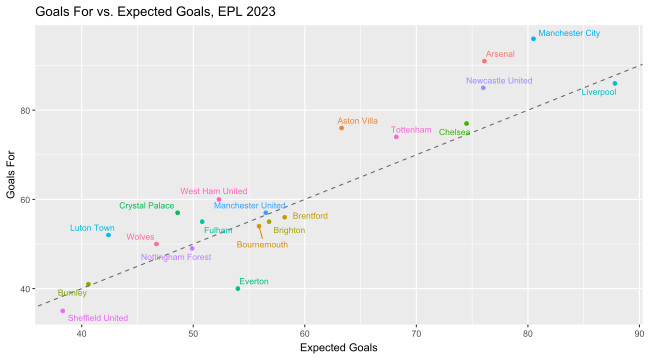
\includegraphics[width=1\linewidth,keepaspectratio=true]{figures/epl_23_g_xg-1} 

}

\caption{Relationship between Goals Scored and Expected Goals by Team (2023-24)}\label{fig:epl_23_g_xg}
\end{figure}

In the chart above, teams above the line are those that over performed,
or those that scored more goals than expected (GF - xG). We can see that
Arsenal counted themselves among the top when it came to expected goals.

\begin{figure}[H]

{\centering 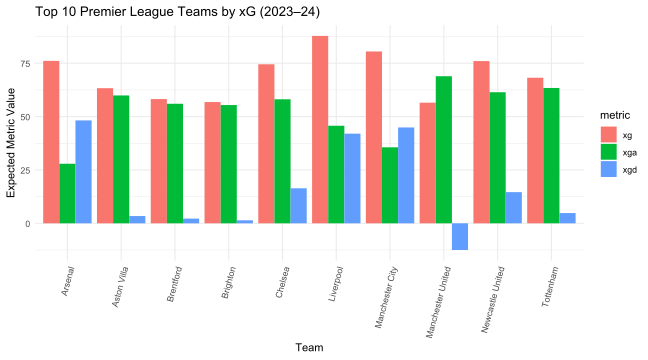
\includegraphics[width=1\linewidth,keepaspectratio=true]{figures/pl_top10_summ-1} 

}

\caption{Expected Goals, Expected Goals Against, and Expected Goal Difference for Top 10 Teams}\label{fig:pl_top10_summ}
\end{figure}

The combination of a strong defence with a budding attacking mindset
would result in an xGD of \textbf{48.2}. Manchester City, on the other
hand, finished the season with an xGD of \textbf{45}, a little lower
than Arsenal's. This naturally drives us towards the question: \emph{do
xG and xGA} \textbf{actually} \emph{correlate to the actual performance
of a team?}.

\begin{figure}[H]

{\centering 
\includegraphics[width=1\linewidth,keepaspectratio=true]{figures/cor_matrix_23-1} 

}

\caption{Correlation Heatmap, Premier League 2023-2024 Season}\label{fig:cor_matrix_23}
\end{figure}

In this heatmap, we can see that for the 2023-2024 season the expected
metrics accurately described a team's performance. The relationship is
particularly strong with \emph{xG} and \emph{Goals For}, showcasing an
\emph{r} of \textbf{0.92}. While not as strong as that of xG-GF,
\textbf{xGA and GA} also show a tight relationship with an \textbf{r} of
\textbf{0.88}. The result then is a tightly related xGD-GD \textbf{r} of
\textbf{0.95}.

Let's again compare the xG-GF relationship, but for the 2024-2025
season. We'll also factor in the previous season's data to see if
there's any observable change or trend and use regression analysis to
support our observations.

\begin{figure}[H]

{\centering 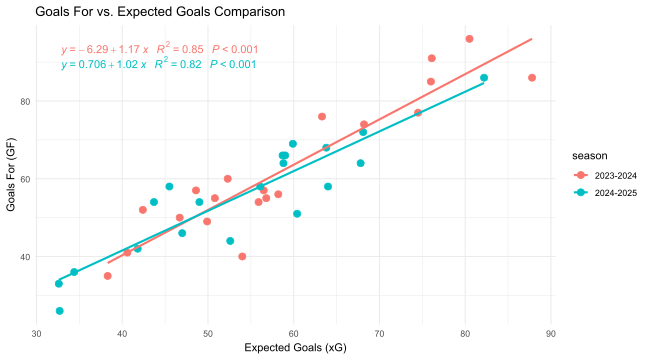
\includegraphics[width=1\linewidth,keepaspectratio=true]{figures/reg_model_xg_gf-1} 

}

\caption{Season-by-Season Comparison of Goals vs Expected Goals with Regression Lines}\label{fig:reg_model_xg_gf}
\end{figure}

Similar to the previous scatterplot comparison, teams above the line are
over performers, and vice versa for those under. The steeper regression
line for the 2023-2024 season hints at a tighter relationship between xG
and GF; the 2024-2025 season's line, while still positive, suggests a
weaker correlation.

\begin{longtable}[]{@{}lrrrr@{}}
\caption{Regression Analysis Summary: Goals For vs Expected Goals
(2023-2025 Seasons)}\tabularnewline
\toprule\noalign{}
term & estimate & std.error & statistic & p.value \\
\midrule\noalign{}
\endfirsthead
\toprule\noalign{}
term & estimate & std.error & statistic & p.value \\
\midrule\noalign{}
\endhead
\bottomrule\noalign{}
\endlastfoot
(Intercept) & -6.2942505 & 6.6180343 & -0.9510755 & 0.3479080 \\
xg & 1.1651818 & 0.1094877 & 10.6421211 & 0.0000000 \\
season2024-2025 & 7.0006734 & 9.3058858 & 0.7522845 & 0.4567709 \\
xg:season2024-2025 & -0.1440598 & 0.1610649 & -0.8944212 & 0.3770377 \\
\end{longtable}

In either case, the relationships are statistically significant and
positive, with p-values and r-squared values supporting the strength of
these correlations. In the table above we can see the exact coefficients
for the regression analysis, where p-values for both seasons are less
than 0.05, which indicates statistical significance. The \(r^2\) value
of \textbf{0.85} implies that approximately \textbf{84.58}\% of the
variance in Goals For (actual goals scored) can be explained by the
Expected Goals (xG) of each team.

Arsenal FC would then end the 2023 campaign with a mean of \textbf{2.39}
goals per match. Combined with an average \textbf{0.76} goals conceded
per match, the team appeared poised for another strong run in the
following season.

\subsection{Defense Wins Championships,
Maybe}\label{defense-wins-championships-maybe}

Which brings us to the actual season in question. As an overview, let's
take a look at the Premier League table at the end of the 2024-2025
season.

\begin{longtable}[]{@{}rlrrrrrr@{}}
\caption{Premier League Table Summary, 2024-2025 Season}\tabularnewline
\toprule\noalign{}
rk & team\_name & gf & ga & gd & pts & xg & xga \\
\midrule\noalign{}
\endfirsthead
\toprule\noalign{}
rk & team\_name & gf & ga & gd & pts & xg & xga \\
\midrule\noalign{}
\endhead
\bottomrule\noalign{}
\endlastfoot
1 & Liverpool & 86 & 41 & 45 & 84 & 82.2 & 38.6 \\
2 & Arsenal & 69 & 34 & 35 & 74 & 59.9 & 34.4 \\
3 & Manchester City & 72 & 44 & 28 & 71 & 68.1 & 47.7 \\
4 & Chelsea & 64 & 43 & 21 & 69 & 67.8 & 47.3 \\
5 & Newcastle United & 68 & 47 & 21 & 66 & 63.8 & 45.5 \\
6 & Aston Villa & 58 & 51 & 7 & 66 & 56.1 & 50.1 \\
7 & Nottingham Forest & 58 & 46 & 12 & 65 & 45.5 & 48.9 \\
8 & Brighton & 66 & 59 & 7 & 61 & 58.7 & 54.6 \\
9 & Bournemouth & 58 & 46 & 12 & 56 & 64.0 & 48.5 \\
10 & Brentford & 66 & 57 & 9 & 56 & 59.0 & 55.4 \\
11 & Fulham & 54 & 54 & 0 & 54 & 49.0 & 47.2 \\
12 & Crystal Palace & 51 & 51 & 0 & 53 & 60.4 & 49.1 \\
13 & Everton & 42 & 44 & -2 & 48 & 41.8 & 46.2 \\
14 & West Ham & 46 & 62 & -16 & 43 & 47.0 & 59.7 \\
15 & Manchester United & 44 & 54 & -10 & 42 & 52.6 & 53.8 \\
16 & Wolves & 54 & 69 & -15 & 42 & 43.7 & 58.1 \\
17 & Tottenham & 64 & 65 & -1 & 38 & 58.8 & 63.3 \\
18 & Leicester City & 33 & 80 & -47 & 25 & 32.6 & 71.9 \\
19 & Ipswich Town & 36 & 82 & -46 & 22 & 34.4 & 72.7 \\
20 & Southampton & 26 & 86 & -60 & 12 & 32.7 & 84.8 \\
\end{longtable}

Again, second place despite having the league's best defensive
structure. Arsenal's defense conceded only \textbf{34} goals throughout
the season, beating the champions Liverpool who conceded \textbf{41}
goals. This only makes it apparent that their difficulties in getting
the ball to the back of the net still outweighed their defensive
capabilities. The team would end the season with a total xG of
\textbf{59.9}, a far cry from last season's \textbf{76.1}.

\begin{figure}[H]

{\centering 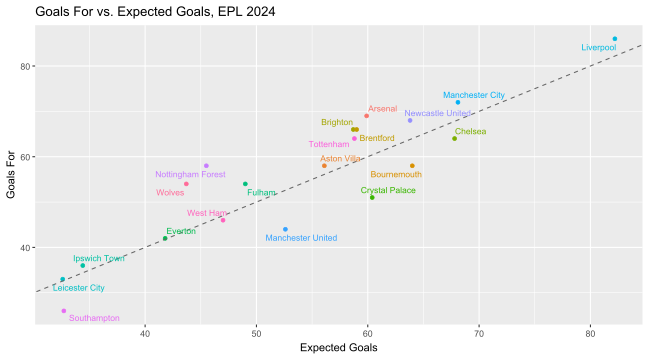
\includegraphics[width=1\linewidth,keepaspectratio=true]{figures/epl_24_g_xg-1} 

}

\caption{Relationship between Goals Scored and Expected Goals by Team (2024-25)}\label{fig:epl_24_g_xg}
\end{figure}

Despite scoring more than their xG, that's still a \textbf{-21.29\%}
change in their expected goal performance, a tell-tale sign that their
chance creation is \textbf{not} what it was. Taking a closer look at the
xG of teams across the league, we can also observe that Arsenal's xG is
the lowest of the top 5 teams.

\subsubsection{Who Needs A Striker?}\label{who-needs-a-striker}

This begs the question; who is responsible for scoring for Arsenal? At
this point in time, Arsenal had its number 9 in the form of Kai Havertz,
a player who \emph{isn't necessarily a traditional striker}. Combined
with their aggressive midfield, we can see where Arsenal pulled most of
its goals from.

\begin{longtable}[]{@{}lrrr@{}}
\caption{Top 5 Arsenal Goal Shares, 2024-2025 Season}\tabularnewline
\toprule\noalign{}
player\_name & goals & goal\_share & cum\_share \\
\midrule\noalign{}
\endfirsthead
\toprule\noalign{}
player\_name & goals & goal\_share & cum\_share \\
\midrule\noalign{}
\endhead
\bottomrule\noalign{}
\endlastfoot
Kai Havertz & 9 & 0.1363636 & 0.1363636 \\
Gabriel Martinelli & 8 & 0.1212121 & 0.2575758 \\
Leandro Trossard & 8 & 0.1212121 & 0.3787879 \\
Mikel Merino & 7 & 0.1060606 & 0.4848485 \\
Bukayo Saka & 6 & 0.0909091 & 0.5757576 \\
\end{longtable}

On this table we have the top 5 goal shares from that season. We can see
that most of the team's goals come from the midfield players with a
total of \textbf{29} goals between them, and Kai Havertz providing a
further \textbf{9} goals on top of that.

In fact, in terms of cumulative shares, Kai Havertz, Gabriel Martinelli,
Leandro Trossard, and Mikel Merino all claim a combined \textbf{48.48\%}
of Arsenal's total goals from 2024-2025. But while these players
threatened the goal when they were on the pitch, injuries would limit
their availability. Let's take a look at the players with the most
minutes:

\begin{longtable}[]{@{}llrrrr@{}}
\caption{Top 5 Arsenal Players by Minutes Played, 2024-2025
Season}\tabularnewline
\toprule\noalign{}
player\_name & position & appearances & minutes & goals & assists \\
\midrule\noalign{}
\endfirsthead
\toprule\noalign{}
player\_name & position & appearances & minutes & goals & assists \\
\midrule\noalign{}
\endhead
\bottomrule\noalign{}
\endlastfoot
David Raya & GKP & 38 & 3420 & 0 & 0 \\
William Saliba & DEF & 35 & 3041 & 2 & 0 \\
Declan Rice & MID & 35 & 2833 & 4 & 7 \\
Thomas Partey & MID & 35 & 2799 & 4 & 0 \\
Leandro Trossard & MID & 38 & 2550 & 8 & 7 \\
\end{longtable}

From this list, only Leandro Trossard provided a big conribution to
Arsenal's total goals. While it could be argued that Declan Rice
provided \textbf{7} assists aside from \textbf{4} goals, his role in the
team is less ``striker'' and more ``controller''. The rest of the
attacking or high scoring players would end up injured, further limiting
Arsenal's goal-scoring edge.

What's important is what we don't see---strikers who \emph{aren't} named
Kai Havertz. With Havertz being the sole striker, the team is reliant on
the German to provide that kind of attacking behavior that midfielders
and wingers don't come naturally with.

Now, let's take into account Arsenal's goal scoring trends over the
season.

\begin{figure}[H]

{\centering 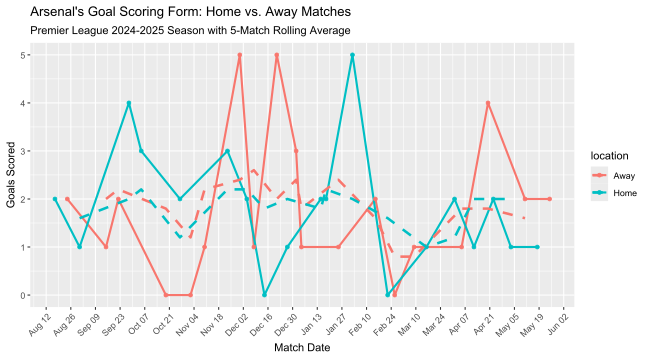
\includegraphics[width=1\linewidth,keepaspectratio=true]{figures/line_10-1} 

}

\caption{Seasonal Goal Scoring Trends by Match Location}\label{fig:line_10}
\end{figure}

With the dashed-line showing the rolling averages, we can see that
Arsenal's scoring form still suffers from inconsistencies. This only
supports the argument that the team just didn't have the depth they
needed to cover for absences caused by injuries.

So can we blame the players? After all, personal challenges could cause
players to underperform. We can break down player attacking
contributions by taking a look at individual player attacking effort and
efficiency. In this scatterplot, the Y-axis shows us the player's
\emph{total attacking contributions} (a sum of their progressive
carries, carries that ended with assists, chances, goals, or shots) and
the X-axis shows us their \emph{pass completion rate}. The size of each
point indicates how many progressive carries that player made throughout
the season.

\begin{figure}[H]

{\centering 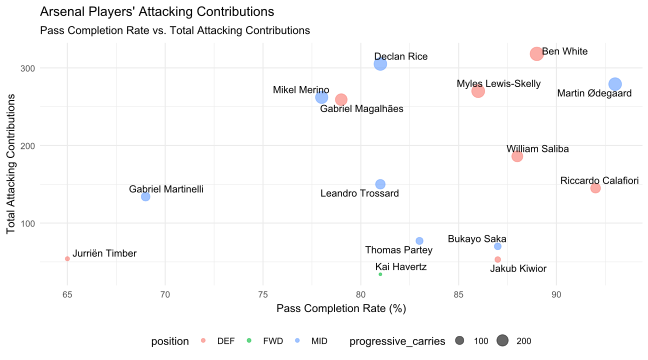
\includegraphics[width=1\linewidth,keepaspectratio=true]{figures/attacking_effort-1} 

}

\caption{Arsenal Players' Attacking Effort: Shots on Target vs Total Shots}\label{fig:attacking_effort}
\end{figure}

With this configuration, we can see that players like Ben White and
Martin Odegaard had high pass completion rates and high attacking
contributions, while players like Kai Havertz and Leandro Trossard had
lower pass completion rates but still contributed significantly to the
team's attacking efforts. In fact, we see a somewhat healthy
distribution of attacking contributions across the squad, across
different positions, indicating that multiple players were involved in
the offensive play.

With that in mind, we can confidently say that the players were actively
trying to make an effort. The following graph shows how efficient each
player is in terms of goal-scoring by comparing their \textbf{goals per
shot on target} against their \textbf{total shots on target}. The size
of each point determines how many goals that player actually scored.

\begin{figure}[H]

{\centering 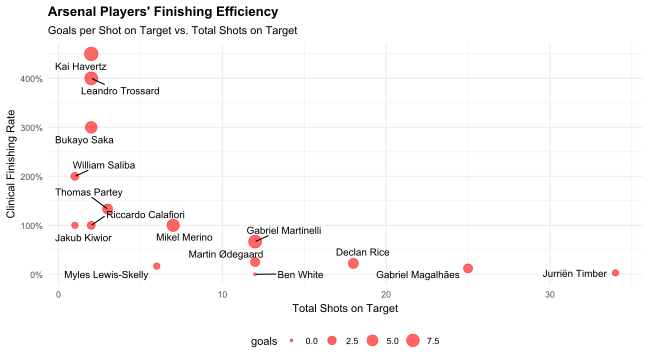
\includegraphics[width=1\linewidth,keepaspectratio=true]{figures/ars_24_conv-1} 

}

\caption{Player-Level Analysis of Finishing Efficiency and Shot Volume}\label{fig:ars_24_conv}
\end{figure}

With the Y-axis showing us the player's \emph{clinical finishing rate}
and the X-axis showing \emph{shots on target}, it's clear that Arsenal's
attacking formation can't hit the target as much as they wanted to. Take
Martin Odegaard, for example; the player is capable of getting into a
position where he can shoot a ball on-target, but the man faces
difficulties getting past the keeper. On the other hand, we have players
like Kai Havertz who only have a few shots on-target but have a high
finishing rate (higher than 100\%!). This is an interesting point with
the data that shows how the definition of a ``Shot on Target'' doesn't
actually define a goal. For example, a player might shoot and ``miss'',
but have the ball deflect into the goal via own-goal.

What we can then derive from the chart is that, while still a capable
team, Arsenal's problem remains the same; they \textbf{need} a number 9,
a traditional striker that converts chances into actual goals.

\subsection{Filling in the Gaps}\label{filling-in-the-gaps}

So, to answer the question of, ``Who needs a striker?'' the answer is
definitely Arsenal. The team has shown a driven desire to improve, and
their defensive record can attest to that. However, without a reliable
goal scorer, the team will continue to struggle to convert their
dominance into actual wins.

\end{document}
